\documentclass[compsoc,draftclsnofoot,onecolumn,10pt]{IEEEtran}
\usepackage[utf8]{inputenc}
\usepackage{color}
\usepackage{url}

\usepackage{enumitem}

\usepackage[letterpaper, margin=.75in]{geometry}
\usepackage{hyperref}
\usepackage{listings}

\usepackage[dvipsnames]{xcolor}
\newcommand*{\SignatureAndDate}[1]{
    \par\noindent\makebox[2.5in]{\hrulefill} \hfill\makebox[2.0in]{\hrulefill}
    \newline\noindent\makebox[2.5in][l]{#1}  \hfill\makebox[2.0in][l]{Date}
}
\usepackage{etoolbox}
\patchcmd{\thebibliography}{\section*}{\subsection}{}{}
\patchcmd{\thebibliography}{\addcontentsline{toc}{section}{\refname}}{}{}{}

\usepackage{graphicx}
\usepackage{float}

\definecolor{dkgreen}{rgb}{0,0.6,0}
\definecolor{gray}{rgb}{0.5,0.5,0.5}
\definecolor{mauve}{rgb}{0.58,0,0.82}

\renewcommand{\lstlistingname}{Code Example} % a listing caption title.

\lstset{
	frame=single,
	language=C,
	columns=flexible,
	numbers=left,
	numbersep=5pt,
	numberstyle=\tiny\color{gray},
	keywordstyle=\color{blue},
	commentstyle=\color{dkgreen},
	stringstyle=\color{mauve},
	breaklines=true,
	breakatwhitespace=true,
	tabsize=4,
	captionpos=b
}

\def\name{Cierra Shawe, Daniel Stoyer, Tao Chen}

%% The following metadata will show up in the PDF properties
\hypersetup{
	colorlinks = false,
	urlcolor = black,
	pdfauthor = {\name},
	pdfkeywords = {ARC,Progress,Report, Fall,2016},
	pdftitle = {Arc Progress Report, Fall 2016},
	pdfsubject = {Progress Report for ARC},
	pdfpagemode = UseNone
}

\def\myversion{1.0 }
\date{}
%
%\usepackage{titlesec}
%
%\usepackage{hyperref}

\parindent = 0.0 in
\parskip = 0.1 in

\setcounter{secnumdepth}{5}

\begin{document}

\begin{titlepage}
\title{
Progress Report\\
\LARGE
ARC - Autonomous RC\\
Senior Capstone Project\\
Oregon State University\\
Fall 2016
}
\author{Tao Chen, Cierra Shawe, Daniel Stoyer}
\maketitle
\begin{center}
	Version 1.0\\
	\today
\end{center}

\thispagestyle{empty} % gets rid of the "0" page number.
	
\end{titlepage}

\tableofcontents

\newpage

\section{Project purpose and goals} 
% Breifly recaps project purpose and goals
The purpose of the Autonomous RC (ARC) project is to determine if it is possible
to build an autonomous RC vehicle using commodity components, meaning components
that are relatively inexpensive and can be bought at places like Radio
Shack\textsuperscript{\textregistered} or Best
Buy\textsuperscript{\textregistered}. \\
Our goal is to make an RC vehicle navigate autonomous to a given
waypoint/location, preferrably at a high rate of speed. Stretch goals are to
make the vehicle drift around corners and parallel park.\\

\[Be sure to add graphic back in before final render!!\]
%\begin{figure}[H]
%   	\includegraphics[width=\textwidth]{autorally_platform_header}
%    \caption{Drifting example. Image from https://autorally.github.io/}
%\end{figure}

While our main goal is to have a functioning autonomous RC vehicle we also hope
that we can produce instructions that RC enthusiasts can follow to produce a
functioning, consumer-grade autonomous RC vehicle of their own.

\section{Current Status}
% Describes where we currently are on the project.

\section{Week-by-week summary of activities}

One thing to note about the following weekly activity summary: if some of our
descriptions seem a bit vague, that is because our understanding of this project
is still fairly vague. We are discovering what we need for this project to
succeed as we go. As the project progresses our focus will narrow and details
will become more concrete. Right now, our understanding of the project is still very
abstract, therefore the concepts and details that we describe are also vague and
somewhat abstract.

\subsection{Weeks 1 - 2}
Weeks one and two were general introduction and orientation weeks. It was
not until week 3 that projects started in earnest and the first assignment was
assigned.

\subsection{Week 3}
	\begin{itemize}
        \item \textit{Activities}:\\
            Worked on creating the problem statement. This required getting an
            overall understanding of what our autonomous RC vehicle should be able
            to do. In other words, getting on paper the expectations of our client
            for the final product. We also started researching what we would need
            for the SRS document, both in terms of the ARC project and in terms of
            the \LaTeX~document. We needed a Gantt chart for the SRS, so we started
            researching how to do that.

        \item \textit{Problems}:\\
            Our client was ill during this time, so feedback for the problem
            statement was understandably delayed. We struggled a little with using
            the proper tense in the document and getting a high-enough, yet detailed
            enough written view of the ARC project. We needed clarification on
            details for the expected vehicle capabilities.

        \item \textit{Solutions}:\\
            We talked with our client on how to frame our project appropriately.
            For the vehicle capabilities, our client told us to aim high, if we
            need to scale things back later we will.

	\end{itemize}
 
\subsection{Week 4}
	\begin{itemize}
        \item \textit{Activities}:\\
            Received feedback on our problem statement and made required
            changes. We needed to clarify what our motivation for the project
            was, namely that we are trying to create an autonomous RC system
            that is considerably less expensive than current research platforms
            (think \$1-2k vs \$10-15k). Created a template for the SRS document
            and started looking into what requirements our project needed.

        \item \textit{Problems}:\\
            The three of us on the ARC team have no prior experience with ECE,
            in general and Autonomy or RC vehicles, in particular. This lack of
            experience makes writing these beginning documents somewhat abstract
            because we do not know what is involved.

        \item \textit{Solutions}:\\
            We spent time with our client to talk through some of the
            requirements. Clarifying why this project matters also helped us
            narrow the scope of our requirements a little bit. We could focus on
            low-cost, readily available components. While that still leaves
            quite a bit to discover, it also eliminates expensive, yet otherwise
            viable, options.

	\end{itemize}
   
\subsection{Week 5}
	\begin{itemize}
        \item \textit{Activities}:\\
            Worked on the SRS document. This phase of the project required us to
            brainstorm what components our system needed and how they fit
            together.\\
            For instance, system interfaces has many parts so we had to sit down
            and talk through what connects and talks to what and visualize how
            that looks. For the SRS, filled out the introduction, software
            interfaces, communications interfaces, and the overall layout of the
            general control flow.\\
            Researched how to construct a Gantt chart in \LaTeX. We also decided
            on what parts we each would take responsibility for and write about
            in the tech review document.

        \item \textit{Problems}:\\
            The SRS document needed different indexing (numeric, as opposed to
            Roman numeral). This required some effort to figure out how to
            reformat the document to use a different indexing scheme without
            changing the controlling document class.\\  
            Other problems: 
            The nature of our project is complex. Therefore,
            there are many parts to the requirements for this project. We needed
            to estimate what the project would need, but again, without
            experience.\\
            Researching and building a working Gantt chart in \LaTeX~took about
            9 hours. The system is very cumbersome, which makes one not want to
            revisit it to make changes.

        \item \textit{Solutions}:\\
            Fixed the \LaTeX~index formatting issue by adding an argument to the
            IEEEtran.cls options. This turned out to be a pretty easy fix, but
            took quite a while to figure out.\\
            We tackled the complexity of this project by meeting together and
            drawing out a rough sketch of major components and how they relate
            to each other.\\

			\[Be sure to add graphic back in before final render!!\]            
%            \begin{figure}[H]
%               	\includegraphics[width=\textwidth]{system_whiteboard_drawing}
%                \caption{White board drawing at first SRS meeting.}
%            \end{figure}

            This gave us a starting point to work from and fill out details for
            what will be required in this project. A big caveat is that these
            are still an \textit{estimate} of requirements. We won't really know
            where we are correct or where we need to add until we get hands-on
            with the hardware and software.\\
            Somewhat mitigated the arduous nature of the \LaTeX~Gantt chart by
            creating a sort of auto-calculation of the percentages for the
            different tasks and sub-tasks.

	\end{itemize}
   
\subsection{Week 6}
	\begin{itemize}
        \item \textit{Activities}:\\
            This was a \textit{very} research-heavy week. We did in-depth
            research on our main areas of emphasis: system interfaces, user
            interfaces, hardware interfaces, communications interfaces, sensors,
            navigation, hardware mounting (how to physically attach the
            components to the vehicle), system control and data processing, and
            path planning. We created a block diagram of the structure and data
            flow of the project.\\

			\[Be sure to add graphic back in before final render!!\]
%            \begin{figure}[H]
%               	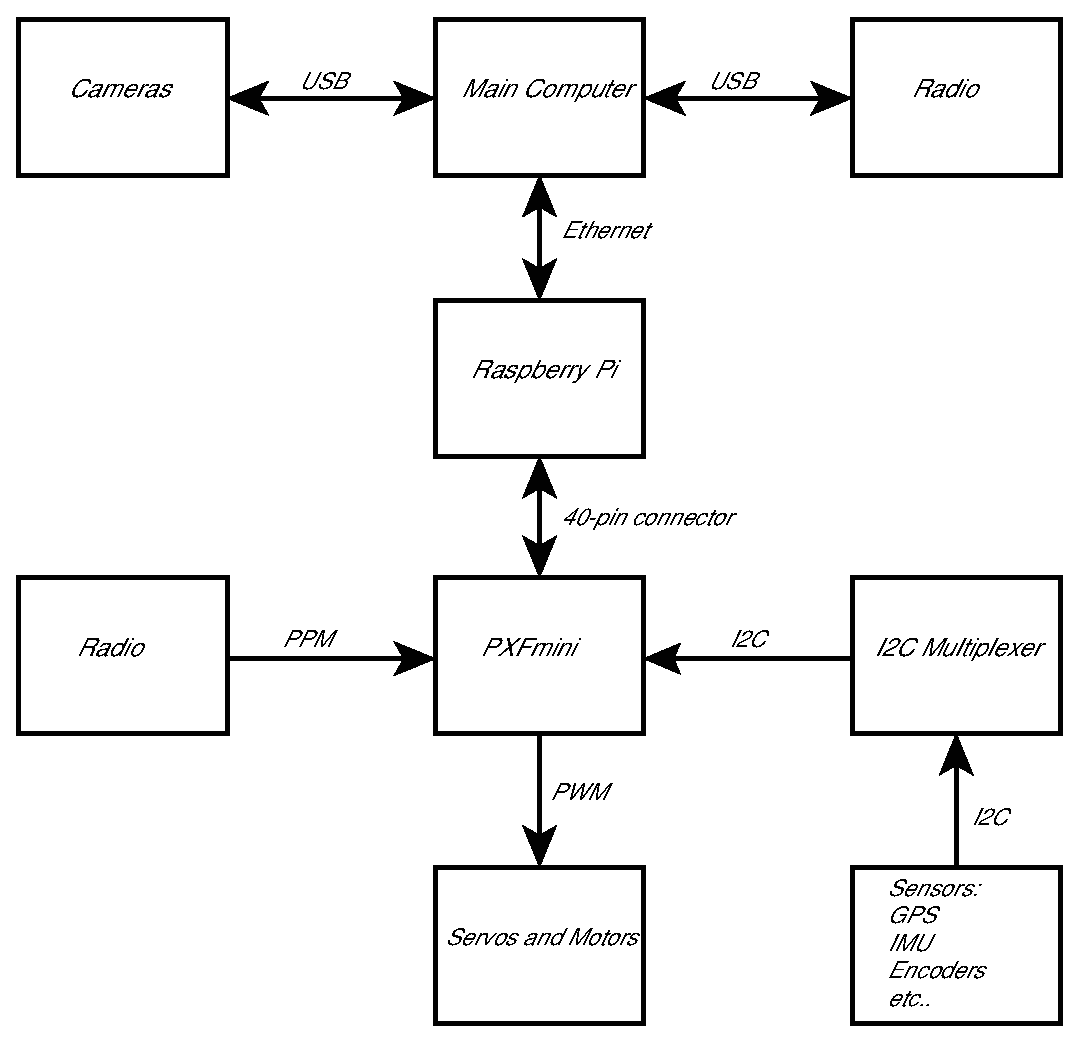
\includegraphics[width=\textwidth]{Block_Diagram}
%                \caption{Structure and data flow of the ARC project}
%            \end{figure}

            We worked simultaneously on the tech review and SRS documents. This
            is likely going to be a better strategy moving forward, research
            some area of the project, determine a requirement based off of the
            research, try to implement, record our findings and adjust the
            requirements further if necessary.

        \item \textit{Problems}:\\
            Which came first, the chicken or the egg? This is how it feels to be
            writing the documents for this research project. In order to know what
            requirements are reasonable/feasible, we need to know what tech is out
            there and if/how it fits with related components.

        \item \textit{Solutions}:\\
            To get around some of the issues we are having we decided to write
            the SRS and the tech review somewhat concurrently. This allowed us
            to research our areas of the tech review and then have a better
            understanding of what a reasonable requirement might be for the
            project.

	\end{itemize}
   
\subsection{Week 7}
	\begin{itemize}
        \item \textit{Activities}:\\
        Fill me in!
        \item \textit{Problems}:\\
        Fill me in!
        \item \textit{Solutions}:\\
        Fill me in!
	\end{itemize}
   
\subsection{Week 8}
	\begin{itemize}
        \item \textit{Activities}:\\
        Fill me in!
        \item \textit{Problems}:\\
        Fill me in!
        \item \textit{Solutions}:\\
        Fill me in!
	\end{itemize}
   
\subsection{Week 9}
	\begin{itemize}
        \item \textit{Activities}:\\
        Fill me in!
        \item \textit{Problems}:\\
        Fill me in!
        \item \textit{Solutions}:\\
        Fill me in!
	\end{itemize}
   
\subsection{Week 10}
	\begin{itemize}
        \item \textit{Activities}:\\
        Fill me in!
        \item \textit{Problems}:\\
        Fill me in!
        \item \textit{Solutions}:\\
        Fill me in!
	\end{itemize}
   
\section{Retrospective}

    % Formatting the table:
    % Each row must be formatted as follows:
    % column 1 & column 2 & column 3\\
    % \hline
    % 
    % Example for text in first column but not in second or third:
    % 
    % some text & & \\
    % \hline
    %
    % Example for text in second column but not in first or third:
	% 
	%  & some text & \\
	% \hline
	%
	% There can be more positives than deltas, but deltas and Actions need to be one-to-one.
    
	\begin{center}
		\begin{tabular}{|p{0.3\linewidth}|p{0.3\linewidth}|p{0.3\linewidth}|}
			\hline
			\textbf{Positives:} & \textbf{Deltas:} & \textbf{Actions:}\\
			
            Anything good that happened. & Changes that need to be implemented. & Specific actions to resolve deltas.\\
			\hline

			Defined our goals for the project. & Design document needs more implementation detail & Winter term add implementation detail.\\
			\hline
			dummy positives & dummy negatives & dummy actions\\
			\hline
			more dummy positives & more dummy negatives & more dummy actions\\
			\hline
			
		\end{tabular}
	\end{center}

\end{document}
